\section{Data Analysis Module for Games}

Blockchain games combine elements of traditional gaming with features of decentralized finance to create a new gaming and economic experience. In this context, on-chain data analysis becomes particularly important as it can offer insights into player behavior, asset liquidity, economic activities, and the health of the gaming ecosystem. Data analysis can bring several key advantages to GameFi projects:
\begin{itemize}
    \item \textbf{Transparency and Verifiability:} Since all transactions and activities are recorded on the blockchain, data analysis can provide fully transparent and verifiable insights into player behavior and economic activities.
\item \textbf{Player Behavior Insights:} Analyzing on-chain data can reveal player preferences, engagement patterns, and behavioral trends, helping developers optimize game design and enhance player experience.
\item \textbf{Economic and Asset Analysis:} Monitoring and analyzing the creation, trading, and liquidity of in-game assets allows developers to better manage the game's economy, preventing inflation or asset value collapse.
\item \textbf{Community and Ecosystem Health:} On-chain data analysis helps assess community activity and engagement, identify key participants and contributors within the ecosystem, thus fostering community growth and sustained engagement.
\end{itemize}

For Carry Protocol, offering data analysis functions in addition to its slot-based advertising features would enable it to provide deeper market insights to game developers and advertisers, optimize advertising strategies, and promote the healthy development of the entire gaming ecosystem. In this way, Carry Protocol can enhance the effectiveness of its advertising platform while supporting the growth and success of GameFi projects through data-driven insights. The framework of Carry data analysis module is illustrated in Figure~\ref{fig:analysis}.

% In the dynamic realm of web3 games, the Carry Protocol recognizes the value of real-time feedback for in-game advertising. Through Performance Benchmark Metrics, the protocol offers immediate insights into the impact and success of each advertising slot. Carry analysis features can be described by Figure \ref{fig:analysis}.

% These metrics don't just offer a retrospective view, they enable active experimentation within games. By analyzing slot performance, developers can refine ad placements, content, and interactivity. This isn't just about placing an ad—it's about optimizing its reach and engagement in a game environment.

% Additionally, these metrics provide a twofold benefit:

% \begin{itemize}
%     \item \textbf{For Game Developers:} They get a clear understanding of how integrated advertisements impact gameplay. This ensures that the core game experience remains uncompromised while still being monetizable.
%     \item \textbf{For Advertisers:} With concrete performance data, advertisers can refine their campaigns. They can tailor content based on which slots garner the most attention, where players spend the most time, and which in-game scenarios drive the most engagement.
% \end{itemize}

% \begin{figure}[!htb]
%     \centering
%     \includegraphics[width=1.0\textwidth]{measurement.png}
%     \caption{Carry Analysis Structure}
%     \label{fig:analysis}
% \end{figure}


% \subsection{Strategy Simulation}


% The Carry Protocol includes a special feature that lets you try out different strategies directly within the blockchain system to see what works best. This tool uses smart contracts, which are like automated rules, to make a secure space for testing. Here, you can change settings and watch how they affect outcomes, helping you make better decisions as you go along.

% Core concepts in experimentation for Carry are:

% \textbf{Variables:} A variable is the basic unit which strategy makers are trying to measure. Whether it's the slot's visibility, its position in the game interface, or the duration of the ad it holds, these variables dictate the behavior of users, regarding certain types of slots. Adjusting them using decentralized logic helps to find the optimal setting for each slot or group of slots.

% \textbf{Groups:} Groups can be a collection of any basic unit in the entire carry protocol, cluster of slots, chosen user addresses, gamers in a certain region etc. Groups are a tool for conducting experiments in a scalable way.

% \textbf{Experiments:} Each 'experiment' revolves around these slots and their groups. Being smart contracts, they execute tests autonomously on these slot configurations. The experiments can range from testing a new slot position to trying out different ad durations. As these experiments run, they yield data, offering insights into the most effective slot configurations.

% \textbf{Rollouts:} Once an experiment concludes, the 'rollouts' come into play. They are the action-driven aftermath of successful experiments, ensuring that proven slot configurations, those variables and group settings that worked, are implemented across the board. It's like upgrading a group of slots based on real, tested data.

% \begin{figure}[!htb]
%     \centering
%     \includegraphics[width=1\textwidth]{experimentation.png}
%     \caption{On-Chain Experimentation made possible with Carry Protocol.}
%     \label{fig:experimentation}
% \end{figure}

% In conclusion, experimentation will greatly help users to measure the performance of their strategies. By enabling experimentation, they ensure that the convergence of games and advertising is not just seamless but also continually evolving, adaptive, and player-centric.

% \subsection{Evaluation Metrics}

% Metrics in the Carry Protocol stand as instrumental indicators, vital in understanding the nuances of in-game advertising in the vast expanse of web3 games. Serving as both compass and map, these metrics provide developers and advertisers with real-time insights into the effectiveness and resonance of each ad slot. Notably, these metrics encompass:

% \begin{itemize}
%     \item \textbf{Actual Views}: Capturing the raw count of users who engage with an ad.
%     \item \textbf{Viewer Profiles}: A snapshot of user demographics, interests, and behaviors, allowing for targeted advertising.
%     \item \textbf{Conversion Metrics}: Indicators that show the transition of viewers from mere observers to engaged participants or customers.
%     \item \textbf{On-chain Payments}: Metrics that display the number of transactions linked to a particular advertisement or slot.
%     \item \textbf{Staking Participation}: Data on users who are not just viewing ads but actively staking their tokens or assets.
%     \item \textbf{Activation Data}: Metrics highlighting the active engagement and interaction of users with an advertisement.
%     \item \textbf{App Installation Data}: Monitoring the number of users who, upon viewing an ad, proceed to install the promoted app.
%     \item \textbf{Community Engagement}: Data on users redirected to and actively participating in the advertised community forums or platforms.
%     \item \textbf{Social Media Engagement}: Monitoring the traction on social media platforms due to the advertisement, gauging the viral potential of ads.
% \end{itemize}

% With these metrics at their fingertips, users can refine their advertisement strategies. They ensure that the ad content doesn't merely inhabit a slot but actively engages, informs, and captivates the game audience, optimizing both visibility and impact.

\subsection{Analysis Objectives}
The evolution of GameFi necessitates a data-driven approach to improve user experience, maintain economic stability, and optimize advertising strategies. Carry Protocol addresses these needs through its robust analytics. The primary objectives can be summarized as follows.
\begin{itemize}
    \item \textbf{Enhancing User Experience:} Analyzing in-game behavior and transaction patterns helps developers understand the user journey. Data reveals which game features captivate players or where they face obstacles. This insight enables developers to iterate on game design, ensuring players find joy and challenge in equal measure, fostering long-term engagement.
\item \textbf{Economic Stability and Inflation Prevention:} Carry Protocol's analytics aim to track the velocity of in-game currencies and the balance between sinks and sources. Monitoring these economic indicators provides the foresight needed to make adjustments that mitigate inflation, keeping the in-game economy vibrant and fair.

\item \textbf{Optimizing Ad Slot Performance:} Advertisement slots are a crucial revenue source in GameFi. Data analysis on slot performance, including user engagement and ad reach, informs strategies to place and design ads that resonate with players without disrupting their gaming experience, ensuring ad slots contribute positively to the game's revenue without detracting from its playability.
\end{itemize}



\begin{figure}[!htb]
    \centering
    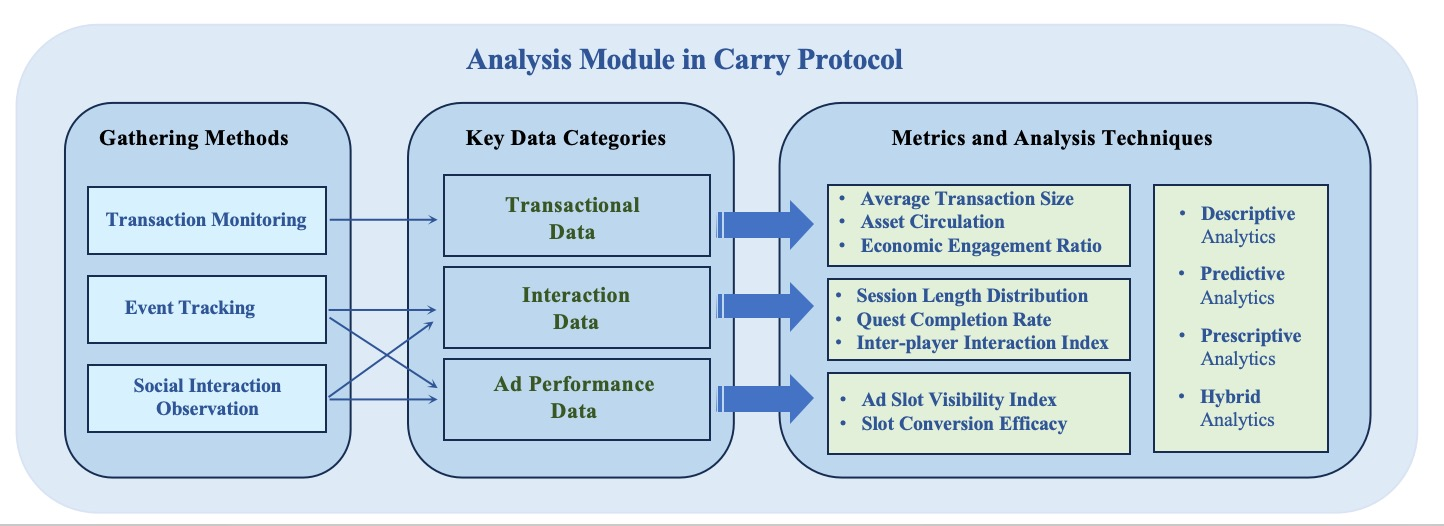
\includegraphics[width=1.0\textwidth]{data analysis.jpg}
    \caption{Data Analysis Framework in Carry Protocol}
    \label{fig:analysis}
\end{figure}



\subsection{Data Types and Metrics}
In this section, we provide detailed data types and significant performance metrics according to the analysis objectives mentioned above.
\subsubsection{Key Data Categories}
For each analytical objective, specific data types are necessary to provide actionable insights.
\begin{enumerate}
    \item \textbf{Transactional Data:} Every in-game transaction, from item purchases to currency exchanges, reflects the game's economic health. Analyzing this data helps in identifying trends, detecting anomalies, and understanding the flow of virtual economies.
\item \textbf{Interaction Data:} Player interactions, both with the game environment and with other players, shed light on community dynamics and engagement levels. This data is invaluable for community management and for enhancing multiplayer aspects of the game.
\item \textbf{Ad Performance Data:} Data on ad views, clicks, and conversions is essential for measuring the effectiveness of in-game advertising. This data category helps advertisers understand the impact of their ads and adjust campaigns for maximum engagement.
\end{enumerate}

\subsubsection{Performance Benchmark Metrics}
% Effective metrics are pivotal for measuring the success of in-game elements and advertising.
% \begin{enumerate}
%     \item \textbf{View Metrics:} These metrics assess how often ads are viewed, offering insights into ad placement and visibility within the game's landscape.
% \item \textbf{Engagement Metrics:} Engagement metrics reveal how players interact with ads, indicating the effectiveness of ad content and design in capturing player attention.
% \item \textbf{Conversion Metrics:}
% Conversion rates measure the success of ads in prompting desired actions, such as in-game purchases or sign-ups, key for evaluating ROI for advertisers.
% \end{enumerate}
Performance Benchmark Metrics within the Carry Protocol are carefully crafted indicators that provide actionable insights derived from specific on-chain data categories. These metrics are designed to evaluate the effectiveness of both the in-game economy and advertising strategies. Here are several refined metrics derived from three aforementioned data types:
\begin{itemize}
    \item \textbf{From Transactional Data:}
    \begin{enumerate}
        \item Average Transaction Size: Indicates the average amount of currency used in transactions, reflecting player spending habits and economic health.
\item Asset Circulation: Measures how frequently in-game assets change hands, revealing the liquidity and dynamism of the game's market.
\item Economic Engagement Ratio: Compares active players to economic transactions, identifying how deeply players are engaged with the in-game economy.
 \end{enumerate}

\item \textbf{From Interaction Data:}
 \begin{enumerate}
     \item Session Length Distribution: Shows the range and average lengths of time players spend in-game per session, indicating engagement depth.
\item Quest Completion Rate: Tracks the percentage of completed in-game quests, measuring content engagement and potential areas for content optimization.
\item Inter-player Interaction Index: Quantifies the interactions between players, such as trades or cooperative play, highlighting the game’s social dynamics.
 \end{enumerate}
\item \textbf{From Ad Performance Data:}
 \begin{enumerate}
\item Player Response Time: Records the time it takes for players to interact with an ad after it appears, indicating the initial impact and relevance of the ad content.
\item Slot Conversion Efficacy: Analyzes the rate at which ad impressions lead to desired player actions, such as in-game purchases or sign-ups, offering a direct measure of ad effectiveness.
 \end{enumerate}
\end{itemize}
The resulting metrics serve distinct purposes.
For Game Developers, they enable fine-tuning of game mechanics to improve player retention, balance the in-game economy, and enhance overall player satisfaction.
For Advertisers, these metrics provide a granular understanding of how different player segments interact with advertisements, informing targeted marketing strategies and creative ad content development. Ultimately, these metrics not only illuminate the current state of game and ad performance but also inform predictions and guide future improvements. They are the linchpin for optimizing GameFi experiences and ensuring that both players and developers reap the maximum benefits from their interactions within the ecosystem.

\subsection{Data Collection and Analysis Techniques}
\subsubsection{Gathering Methods}
The granularity and accuracy of data collection determine the quality of insights derived. 
\begin{itemize}
    \item \textbf{Event Tracking:} This method is leveraged for player interaction data, including player actions, in-game achievements, quest completions, etc. Capturing in-game events provides a detailed picture of player behavior and game mechanics efficacy, allowing for granular analysis and immediate feedback for iterative development. Through an SDK or API integrated into the game client, player operations and game events are captured in real-time. Then, each event is tagged and categorized for deep analysis, such as player progress, preferences, and areas of friction.
\item \textbf{Transaction Monitoring:} This method is leveraged for economic activity data, encompassing player-to-player transactions, purchases of virtual items, currency liquidity, etc. By real-time recording and indexing of all in-game and inter-game transactions using smart contracts and blockchain event logs, Carry Protocol can provide real-time data on economic activities, facilitating a responsive approach to economic management within the game. Finally, it enables developers to monitor and adjust in-game economic policies, prevent inflation, and ensure the health and sustainability of the game economy. Figure~\ref{fig:monitoring} introduced by \href{https://www.wipro.com/blockchain/monitoring-and-management-of-blockchain-networks/}{wipro} represents a blockchain monitoring framework.

\begin{figure}[!htb]
    \centering
    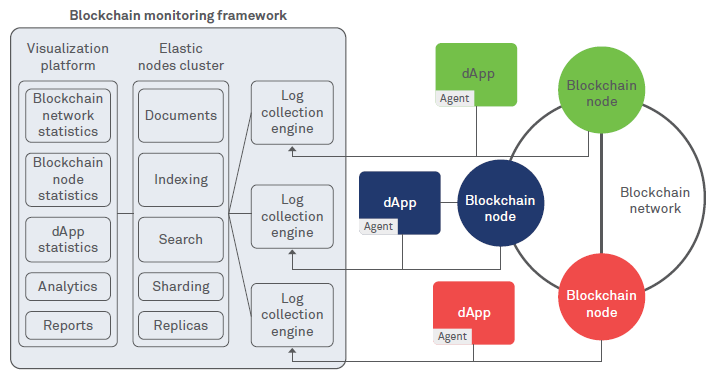
\includegraphics[width=0.9\textwidth]{monitoring-and-management-of-blockchain-networks-2.png}
    \caption{Transaction Monitoring Framework}
    \label{fig:monitoring}
\end{figure}
\item \textbf{Social Interaction Observation:} This method is leveraged for community engagement data, such as communications between players, collaboration, and formation of social networks within the game.
These data collected by analyzing players' in-game chat logs, teamwork, and social interaction events.
Insights into the community's vibrancy, social structure, and player engagement levels can be gleaned from social interaction data. Developers can design more attractive social features and events based on these insights, encouraging interaction and collaboration among players.
\end{itemize}

\subsubsection{Analytical Methodologies}
Each data type requires a specific analysis approach to transform raw data into meaningful insights.
\begin{itemize}
    \item \textbf{Descriptive Analytics:}
This foundational method summarizes raw data into interpretable formats, establishing a baseline understanding of in-game and economic activities. For example, we can aggregating transactional data to compute average transaction size, volume, and frequency over specific time intervals. By analyzing these aggregates, developers can understand the peak times of economic activity within the game, identify spending patterns, and potentially discover underutilized areas of the game economy that could be developed further.
\item \textbf{Predictive Analytics:}
Using statistical models and machine learning algorithms, predictive analytics forecasts future trends, informing proactive game and economic development strategies. For example, we can employ machine learning models, such as decision trees or neural networks, to predict player churn based on interaction data like session length, frequency of play, and engagement in community events. These predictions enable developers to proactively implement features or incentives aimed at retaining players at higher risk of churn, effectively increasing overall engagement and player lifetime value. For example, \href{https://cloud.google.com/blog/topics/developers-practitioners/churn-prediction-game-developers-using-google-analytics-4-ga4-and-bigquery-ml}{Google Cloud} proposed to use BigQuery ML on the sample app dataset to predict propensity to user churn or not churn based on users' demographics and activities within the first 24 hours of app installation.
\begin{figure}[!htb]
    \centering
    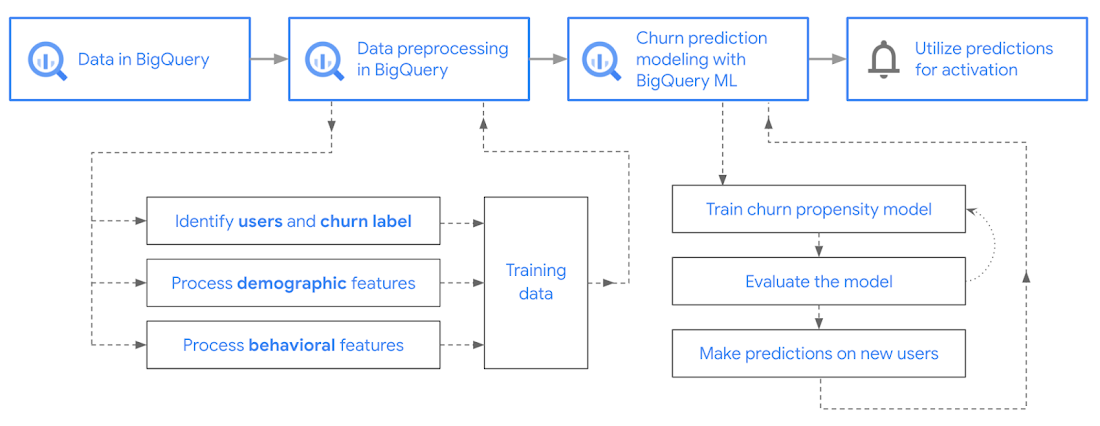
\includegraphics[width=1\textwidth]{prediction.png}
    \caption{Predictive Analytics Framework Proposed by Google Cloud}
    \label{fig:prediction}
\end{figure}
\item \textbf{Prescriptive Analytics:}
Beyond predicting future trends, prescriptive analytics suggests concrete actions to achieve desired outcomes, such as improving user retention or optimizing ad placements. For example, we can utilize advanced analytics, such as optimization algorithms or simulation models, to analyze click-through rates (CTR), conversion rates (CR), and ad exposure duration across different player segments.
Insight: This analysis can suggest which ad content is most effective for specific player demographics or in-game contexts, guiding advertisers on how to tailor their campaigns. For example, if certain ad placements consistently lead to high conversion rates among players who enjoy PvP content, similar strategies can be applied to target this player segment more effectively.
\item \textbf{Combining Methodologies for Comprehensive Insights:} By integrating descriptive, predictive, and prescriptive analytics, Carry Protocol can offer a holistic view of the game's ecosystem. For instance, descriptive analysis of transactional data may reveal an increasing trend in virtual item purchases. Predictive analytics could then forecast this trend's continuation based on current game dynamics and player behavior. Finally, prescriptive analytics could recommend specific in-game events or promotions to capitalize on this trend, such as limited-time offers on popular items or introducing new items likely to be popular based on player preferences inferred from past data.

\end{itemize}

By addressing these objectives, categories, and methodologies, Carry Protocol's data analysis SDK will empower developers and advertisers with the tools needed to unlock the full potential of GameFi. This structured approach ensures that every facet of the gaming experience and economy can be analyzed, optimized, and enhanced for the benefit of all stakeholders in the ecosystem.